\Needspace{12\baselineskip}
\section{Critical behavior and finite-size predictions}
\label{sec:theoretical-predictions}

The models in \cref{sec:models-and-observables} specify how to draw a graph.
We now ask what fraction of its vertices can remain after repeated deletion,
and how that prediction changes near the transition. There are three levels
of justification: established CM core theorems, deductions from the triangle
cavity equations, and a proposed finite-size approximation for triangles.
Keeping these separate is essential when comparing the predictions with data.

\subsection{Configuration-model equations and theorems}
\label{sec:configuration-theory}

An edge can help retain its other endpoint only if the vertex supplying that
connection has at least two further surviving connections. Imagine keeping
the receiving endpoint present while testing this condition. Let $x$ be the
probability that a directed edge supplies such support. This conditional
question is called a cavity calculation: the contribution of the receiving
edge is excluded while counting the other available connections.

Write $K$ for the limiting CM degree, with probabilities $\pi_k$ from
\cref{eq:limiting-degree-law}, and let $\mu=\E[K]=2\lambda$.
Following a uniformly chosen edge reaches a degree-$k$ vertex with probability
$k\pi_k/\mu$, because it has $k$ possible incident ends. This is the
\emph{size-biased} degree law. For fixed $\lambda>0$, a bounded neighbourhood
of the CM becomes a tree as $n$ grows. Its different outward branches are
independent in the limit. Given degree $k$, the number of other supporting
edges is therefore $\operatorname{Bin}(k-1,x)$, a binomial variable with
$k-1$ trials and success probability $x$. Consequently
\begin{equation}
  x=F_\lambda(x):=
  \sum_{k\geq1}\frac{k\pi_k}{\mu}
  \Prob\{\operatorname{Bin}(k-1,x)\geq2\}.
  \label{eq:cm-support}
\end{equation}
At a uniformly chosen vertex all $k$ incident edges are available, giving
\begin{equation}
  \mathcal R_{\mathrm{CM}}(x,\lambda)=
  \sum_{k\geq0}\pi_k\Prob\{\operatorname{Bin}(k,x)\geq3\}.
  \label{eq:cm-density-sum}
\end{equation}
The predicted density is $\rho_{\mathrm{CM}}(\lambda)=
\mathcal R_{\mathrm{CM}}(x(\lambda),\lambda)$ at the selected solution.

These sums have short closed forms. The function
$G_0(t)=\E[t^K]=\exp\{\lambda(t^2-1)\}$ encodes the degree probabilities as
its coefficients. The corresponding function after following an edge is
$G_1(t)=G_0'(t)/\mu=t\exp\{\lambda(t^2-1)\}$.
The probabilities of zero and one successes are $G_1(1-x)$ and
$xG_1'(1-x)$. Subtracting them from one gives
\begin{equation}
  F_\lambda(x)=1-e^{-\lambda x(2-x)}
  [1+2\lambda x(1-x)^2].
  \label{eq:cm-support-closed}
\end{equation}
For the density, subtract the probabilities of zero, one, and two successes
using $G_0$, $xG_0'$, and $x^2G_0''/2$:
\begin{equation}
 \begin{split}
  \mathcal R_{\mathrm{CM}}(x,\lambda)
  =1-e^{-\lambda x(2-x)}\big[&1+2\lambda x(1-x)\\
    &+\lambda x^2+2\lambda^2x^2(1-x)^2\big].
 \end{split}
 \label{eq:cm-density}
\end{equation}

The zero solution always exists. To select the solution corresponding to
pruning, start with all connections available, $x_0=1$, and repeatedly set
$x_{t+1}=F_\lambda(x_t)$. Since $F_\lambda$ is increasing, this sequence
decreases to its largest fixed point. Starting at zero would miss a
positive core. Above the critical point, the CM law of large numbers
identifies \cref{eq:cm-density} at this largest, crossing root as the
limiting core fraction; below it the fraction tends to zero
\cite[Condition~2.2 and Theorem~2.3]{janson2007kcore}.
The twice-Poisson degrees satisfy the required degree and moment conditions.
That theorem's crossing condition fails at the critical tangency, so it
does not assign a deterministic density there. Critical fluctuations require
\cref{sec:fluctuation-scales} instead. At $\lambda=0$ both models are edgeless
and their core fractions are zero.

\subsection{Joint cavity equations for triangles}
\label{sec:triangle-cavity}

The triangle graph contains short cycles even as $n$ grows. Its two
neighbours in one community are connected, so treating their edges as
independent would change the pruning problem. Instead, retain the incidence
representation from \cref{sec:triangle-model}. Its local limit is a tree
of individual and community vertices~\cite[Theorem~2.14]{hofstad2021communities}.
Independence then applies between separate outward community branches.

Following a membership reaches an individual with membership count $D^*$
weighted in proportion to its count. For $D\sim\operatorname{Poisson}(\lambda)$,
\begin{equation}
  \Prob(D^*-1=j)=\frac{(j+1)\Prob(D=j+1)}{\lambda}
  =e^{-\lambda}\frac{\lambda^j}{j!}.
  \label{eq:poisson-excess-memberships}
\end{equation}
Thus both a root and an individual reached through one community have a
Poisson number of available other communities, with mean $\lambda$.

Consider a triangle containing $v,u_1,u_2$, and temporarily keep $v$ present.
Let $S_i$ count neighbours offered to $u_i$ through other communities,
evaluated with $u_i$ itself kept available. Let $J\in\{0,1,2\}$ count how many
of $u_1,u_2$ can remain
jointly and thus supply neighbours to $v$. If both $S_i\geq1$, both remain:
each has the other two triangle vertices and an external neighbour.
If one $S_i=0$, that individual is deleted, and the other remains exactly
when its external count is at least two. All other cases give $J=0$.
This local calculation retains the edge between $u_1$ and $u_2$ throughout;
it does not demand that an entire triangle survive.

Write $q_j=\Prob(J=j)$ and $p_j=\Prob(S=j)$, where $S$ is the external
support count on one limiting branch. Independence of the two external
branches gives
\begin{equation}
  \begin{gathered}
    q_2=(1-p_0)^2,\qquad q_1=2p_0(1-p_0-p_1),\\
    q_0=1-q_1-q_2.
  \end{gathered}
  \label{eq:triangle-messages}
\end{equation}
A vertex receives a Poisson number of these messages. The counts of messages
of sizes one and two are independent Poisson variables with means
$\lambda q_1$ and $\lambda q_2$. Therefore $S$ has the distribution of
$A+2B$, where $A\sim\operatorname{Poisson}(\lambda q_1)$ and
$B\sim\operatorname{Poisson}(\lambda q_2)$ are independent. Enumerating the
ways to obtain support zero, one, or two yields
\begin{equation}
 \begin{aligned}
  p_0&=e^{-\lambda(q_1+q_2)},& p_1&=\lambda q_1p_0,\\
  p_2&=\left[\lambda q_2+\tfrac12(\lambda q_1)^2\right]p_0.
 \end{aligned}
 \label{eq:triangle-closure}
\end{equation}
Together, \cref{eq:triangle-messages,eq:triangle-closure} close the equations
in $(q_1,q_2)$. A root survives when its total support is at least three, so
\begin{equation}
  \mathcal R_\triangle(q,\lambda)=1-p_0-p_1-p_2,
  \qquad q=(q_1,q_2).
  \label{eq:triangle-density}
\end{equation}

Pruning starts with every triangle offering two neighbours, $(q_1,q_2)=(0,1)$.
Iterate the probability update from that state. The quantities that decrease
are the tails $q_1+q_2=\Prob(J\geq1)$ and $q_2=\Prob(J\geq2)$;
$q_1$ alone can increase when two supports become one. Monotonicity of the
local deletion rule makes this iteration select the largest message law in
these two tails, and hence the physical density prediction.

The calculation is exact for the stated local rule on the limiting incidence
tree. Using it for the finite graph's terminal core additionally assumes that
the large-graph limit can be combined with arbitrarily many pruning rounds.
Local convergence controls each fixed depth, and does not establish that
interchange. We call the resulting $\rho_\triangle(\lambda)$ a cavity
prediction. Motif-aware core calculations provide related context
\cite{bhat2017clustered}, but do not supply a fluctuation theorem for this
particular ensemble.

\subsection{Critical points and the saddle-node expansion}
\label{sec:transition-criteria}

A positive solution first becomes available when two solution branches meet
at a turning point, called a saddle-node. For the CM set
$\mathcal G_{\mathrm{CM}}(x,\lambda)=F_\lambda(x)-x$. Its critical point
satisfies
\begin{equation}
  F_{\lambda_c}(x_c)=x_c,\qquad
  \partial_xF_{\lambda_c}(x_c)=1.
  \label{eq:cm-criticality}
\end{equation}
For fixed $x\in(0,1)$, $F_\lambda(x)$ increases strictly with $\lambda$.
Solving $F_\lambda(x)=x$ defines a parameter curve $\Lambda(x)$ whose
interior minimum gives \cref{eq:cm-criticality}. Its parameter diverges at
both ends. Moreover $F_\lambda(x)=(3\lambda+2\lambda^2)x^2+O(x^3)$ near zero,
so a positive root cannot merge continuously with zero at finite $\lambda$.
The unique critical contact and its nonzero curvature are justified in
\cref{app:support-calculations}.

For triangles, eliminate the two message probabilities by putting
$u=p_0=e^{-z}$, $z>0$. At a fixed point,
\begin{equation}
 q_2=(1-u)^2,\qquad q_1=\frac{2u(1-u)}{1+2\lambda u^2}.
 \label{eq:triangle-scalar-messages}
\end{equation}
The remaining equation is
\begin{equation}
  \mathcal G_\triangle(z,\lambda)=H(z,\lambda)
  :=\lambda(q_1+q_2)-z=0.
  \label{eq:triangle-scalar}
\end{equation}
Its derivative $H_\lambda=(1-u)^2+2u(1-u)/(1+2\lambda u^2)^2$ is positive.
Multiplying by $1+2\lambda u^2$ gives a quadratic in $\lambda$, whose positive
root is
\begin{equation}
 \begin{split}
  \Lambda(z)&=\frac{2z}{B(z)+\sqrt{B(z)^2+8u^2(1-u)^2z}},\\
  B(z)&=1-u^2-2u^2z,\qquad u=e^{-z}.
 \end{split}
 \label{eq:triangle-parameter-curve}
\end{equation}
Every positive solution lies on this curve. At fixed $\lambda$, larger $z$
means larger values of both $q_2$ and $q_1+q_2=z/\lambda$, so the largest
$z$ root gives the pruning-selected law. The criticality equations are
$H(z_c,\lambda_c)=H_z(z_c,\lambda_c)=0$.
Since $\Lambda(z)\sim(2z)^{-1/2}$ near zero and $\Lambda(z)\sim z$ at infinity,
the first solution occurs at a positive interior minimum. The update
Jacobian at zero is $\left(\begin{smallmatrix}0&2\lambda\\0&0\end{smallmatrix}\right)$;
its eigenvalues are zero, excluding a finite-parameter merger with the zero
solution. The predicted density at onset is therefore positive.
The observed single-fold shape of the explicit triangle curve is numerically
checked; an analytic uniqueness theorem is not claimed.

For either model write $y=x$ or $z$ for its scalar coordinate and
$\mathcal R_M(y,\lambda)$ for its density map, composing
\cref{eq:triangle-scalar-messages} with \cref{eq:triangle-density} for triangles.
All derivatives below hold the other argument fixed. At the critical point
both models have
\begin{equation}
  \begin{gathered}
    \mathcal G_M=\mathcal G_{M,y}=0,\\
    \mathcal G_{M,\lambda}>0,\quad \mathcal G_{M,yy}<0,\quad
    \mathcal R_{M,y}>0.
  \end{gathered}
  \label{eq:fold-conditions}
\end{equation}
Let $\delta=\lambda-\lambda_c>0$ and $v=y-y_c$. Taylor expansion gives
\begin{equation}
 \begin{split}
  0={}&\mathcal G_{M,\lambda}\delta+\tfrac12\mathcal G_{M,yy}v^2\\
    &+O(\delta^2+|v|\delta+|v|^3).
 \end{split}
 \label{eq:fold-taylor}
\end{equation}
The larger branch consequently has
$v=b_M\sqrt\delta+O(\delta)$, where
$b_M=\sqrt{-2\mathcal G_{M,\lambda}/\mathcal G_{M,yy}}$.
Expanding the density in turn gives the required result:
\begin{equation}
 \begin{split}
  \rho_M(\lambda)&=\rho_{c,M}+a_M\sqrt{\lambda-\lambda_{c,M}}
                    +O(\lambda-\lambda_{c,M}),\\
  a_M&=\mathcal R_{M,y}
       \sqrt{-2\mathcal G_{M,\lambda}/\mathcal G_{M,yy}}.
 \end{split}
 \label{eq:density-square-root}
\end{equation}
Here $\rho_{c,M}>0$ is the positive branch's right-hand limit, distinct from
the zero solution below the threshold. The direct dependence of
$\mathcal R_M$ on $\lambda$ contributes only at order $\delta$.
Thus a coefficient derived for a message coordinate must be multiplied by
$\mathcal R_{M,y}$ before predicting a core fraction.

\begin{table}[tb]
  \centering
  \caption{Critical values and density coefficients computed from the model
    equations. The triangle row is a cavity prediction. Digits express
    numerical precision for these equations, not finite-graph accuracy.}
  \label{tab:critical-predictions}
  % Generated by notebooks/theory_comparison.ipynb; regenerate with make theory-figures.
\begin{tabular}{lrrr}
\toprule
Model & $\lambda_c$ & $\rho_c$ & $a$ \\
\midrule
CM multigraph & 1.287720 & 0.137889 & 0.317959 \\
Triangle cavity & 1.228598 & 0.081112 & 0.278553 \\
\bottomrule
\end{tabular}

\end{table}

The numerical procedure first brackets the minimum of $\Lambda$ and then
bisects its derivative, rather than reporting a grid point as the threshold.
For CM, implicit differentiation gives
$\Lambda'=(1-\partial_xF_\lambda)/(\partial_\lambda F_\lambda)$;
for triangles it gives $\Lambda'=-H_z/H_\lambda$.
Above the fold, bisection on the larger-coordinate side selects the positive
branch. Residuals in the original equations check the result.
\Cref{tab:critical-predictions} records the evaluated constants.
Analytic derivative formulas are given in \cref{app:support-calculations}.
Independent centred differences and direct branch solutions verify them:
$[\rho_M(\lambda_c+\delta)-\rho_c]/\sqrt\delta$ approaches $a_M$, while the
unscaled remainder is of order $\delta$.
\Cref{fig:theory-fold} shows both the jump and this local limit.
The near-double root magnifies roundoff at extremely small offsets, so the
checks use a sequence of resolvable offsets and derivative step sizes
(\cref{app:numerical-checks}).

\begin{figure*}[tb]
  \centering
  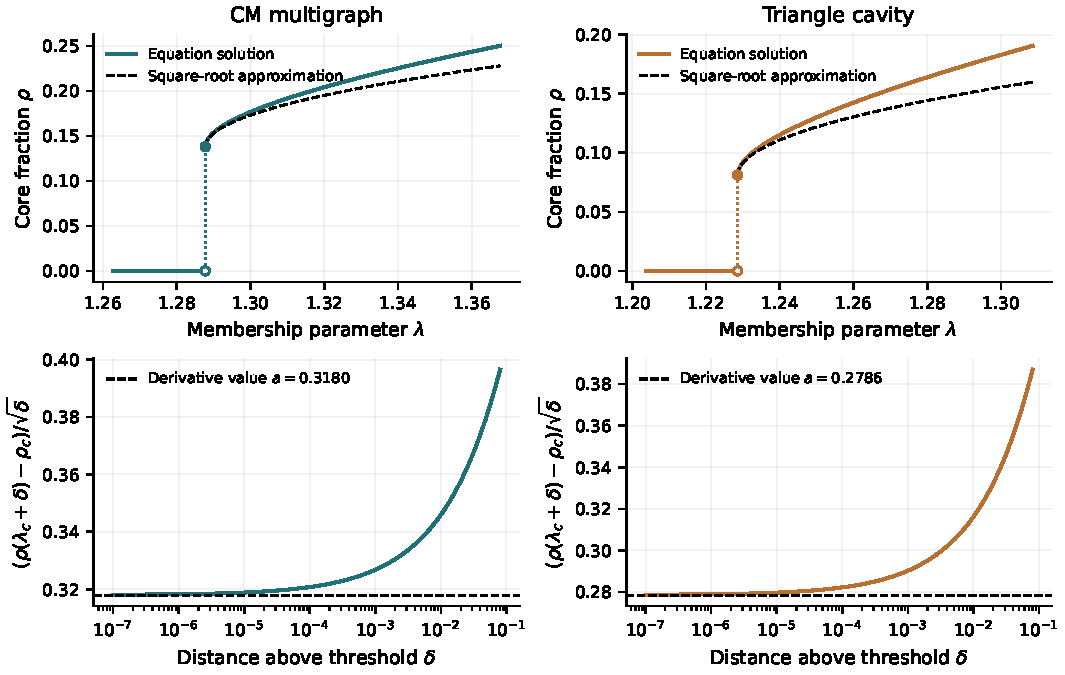
\includegraphics[width=\textwidth]{theory_fold_comparison.pdf}
  \caption{Deterministic theory near the transition. Upper panels compare the
    maximal-branch density with its leading square-root approximation. Dotted
    vertical segments indicate jumps from the separate zero branch; filled
    markers denote the positive right-hand limits. Lower panels divide the
    density increase by $\sqrt\delta$, where $\delta=\lambda-\lambda_c>0$.
    The ratios approach the derivative-based coefficients (dashed lines),
    while higher-order terms become visible farther above onset. No graph
    simulations or fitted density parameters enter this figure.}
  \label{fig:theory-fold}
\end{figure*}

\subsection{Critical windows and fluctuation scales}
\label{sec:fluctuation-scales}

Finite graphs with identical $n$ and $\lambda$ need not produce the same core.
Their sampled memberships differ, and even fixed memberships can be matched
differently. Near a turning point, a small perturbation can either leave a
positive branch available or remove it altogether. This motivates treating
the distance from criticality as a random quantity.

The CM supplies an established benchmark for this reasoning. The appropriate
results are the prescribed-degree critical theorem and the random-degree
conditioning argument of \cite[Theorem~3.5 and Section~8]{janson2008fluctuations}.
Its Erd\H{o}s--R\'enyi-specific constants cannot be used for twice-Poisson degrees.
Here is their specialization to our retained CM, with the checks and variance
calculation detailed in \cref{app:support-calculations}.

Let $\lambda_n=\lambda_c+u/\sqrt n$ for a fixed real offset $u$.
For a prescribed degree $k$, put
$h_k(x)=\E[Y\mathbf1_{\{Y\geq3\}}]$, where $Y\sim\operatorname{Bin}(k,x)$
and $\mathbf1$ is the indicator of the stated event.
In the theorem's auxiliary pruning process, the expected number of remaining
edge ends per input vertex is the mean degree times $x^2$.
The quantity $h_k(x)$ counts ends at vertices with at least three remaining
ends. Their difference counts ends at vertices still eligible for deletion.
Running out of such ends can stop the process with a positive core.
The corresponding empirical difference is
\begin{equation}
  \ell_n(x)=\frac1n\sum_{i=1}^n[K_i x^2-h_{K_i}(x)].
  \label{eq:empirical-bottleneck}
\end{equation}
Its population version is
$\ell(x,\lambda)=2\lambda x[x-F_\lambda(x)]$.
At $(x_c,\lambda_c)$ it has a quadratic minimum. Define
$c=-\partial_\lambda\ell(x_c,\lambda_c)>0$ and
$\beta=\partial_x^2\ell(x_c,\lambda_c)>0$.
The first measures the change in the minimum's height with $\lambda$;
the second measures its curvature.

Sampling the degrees makes the minimum fluctuate: if $\bar x_n$ is its
nearby minimizer, then
\begin{equation}
  \sqrt n\,\ell_n(\bar x_n)\xrightarrow{d}-cu+U,
  \qquad U\sim N(0,v_{\mathrm{degree}}).
  \label{eq:degree-noise}
\end{equation}
The pruning theorem adds an independent centred Gaussian contribution from
pairing, with variance $v_{\mathrm{pair}}$. For our degree law the two evaluated
variances are approximately $0.249099$ and $0.107879$, respectively.
Set
\begin{equation}
  \tau_{\mathrm{CM}}=
  \frac{\sqrt{v_{\mathrm{degree}}+v_{\mathrm{pair}}}}{c}
  \approx1.95625.
  \label{eq:cm-noise-scale}
\end{equation}
Let $Z\sim N(0,1)$ and $W=u+\tau_{\mathrm{CM}}Z$.
Writing $Y_{n,\mathrm{CM}}=
n^{1/4}(R_{n,\mathrm{CM}}-\rho_{c,\mathrm{CM}})$, the critical-window limits become
\begin{equation}
 \begin{split}
  \Prob(A_{n,\mathrm{CM}}(\lambda_n))
    &\longrightarrow\Phi(u/\tau_{\mathrm{CM}}),\\
  Y_{n,\mathrm{CM}}\mid A_{n,\mathrm{CM}}
    &\xrightarrow{d}a_{\mathrm{CM}}\sqrt W\mid\{W>0\}.
 \end{split}
 \label{eq:cm-critical-limit}
\end{equation}
Here $\Phi$ is the standard normal distribution function and
$\xrightarrow{d}$ denotes convergence in distribution.
Any fixed cutoff $0<\varepsilon_{\mathrm{CM}}<\rho_{c,\mathrm{CM}}$ selects
the same asymptotic substantial-core event. Both sources of randomness matter:
using pairing noise alone would give a different limit for the existing
experiments, which resample degrees on every trial.

For triangles, suppose the scalar equation has a random perturbation of
order $n^{-1/2}$ near its fold. Writing its leading noise as
$n^{-1/2}\xi$ in \cref{eq:fold-taylor} replaces $\delta$ by
$\delta+n^{-1/2}\xi/\mathcal G_{M,\lambda}$.
If the scaled perturbation has a nondegenerate limiting distribution, a
change in $\lambda$ of order $n^{-1/2}$ competes with it. The fold then turns
this into a coordinate and density displacement of order $n^{-1/4}$ on
surviving outcomes. Thus we test a window of width $O(n^{-1/2})$ and
\begin{equation}
  R_{n,M}-\rho_{c,M}=O_p(n^{-1/4})\ \text{conditional on }A_{n,M}.
  \label{eq:conditional-scaling}
\end{equation}
The notation means that $n^{1/4}(R_{n,M}-\rho_{c,M})$ stays bounded in
probability under the conditional laws. Multiplying by $n$ gives core-count
fluctuations of order $n^{3/4}$ about $n\rho_{c,M}$.
These statements apply within the critical window, not at every parameter.
Unconditionally, the distribution also contains outcomes near zero, far
from $\rho_c$. Neither the noise order nor Gaussianity follows from the
deterministic square root. They are additional triangle hypotheses;
local incidence convergence proves neither. The CM constants also do not
automatically apply to its erased projection.

\subsection{A stochastic prediction for surviving core sizes}
\label{sec:stochastic-approximation}

To obtain a prediction that can be tested without fitting the sizes it aims
to explain, let survival observations determine an effective threshold's
centre and spread. For each $n,M$, let $\mu_{n,M}$ be its centre in membership
parameter units and $w_{n,M}>0$ its width. Propose the occurrence curve
\begin{equation}
  \Prob(A_{n,M}(\lambda))\approx
  \Phi\!\left(\frac{\lambda-\mu_{n,M}}{w_{n,M}}\right).
  \label{eq:occurrence-model}
\end{equation}
This is equivalent to a normal random effective threshold. At a given
$\lambda$, abbreviate
$m=\sqrt n(\lambda-\mu_{n,M})$ and $s=\sqrt n\,w_{n,M}$, and define
\begin{equation}
  V=m+sZ,\qquad Z\sim N(0,1).
  \label{eq:random-distance}
\end{equation}
The approximation identifies survival with $V>0$. Its conditional density
prediction is
\begin{equation}
  Y:=n^{1/4}(R_{n,M}-\rho_{c,M})\mid A_{n,M}
  \ \approx\ a_M\sqrt V\mid\{V>0\}.
  \label{eq:stochastic-fold}
\end{equation}
The same random distance explains both whether a core appears and how much
its fraction exceeds the jump. Theory supplies $\rho_{c,M}$ and $a_M$;
only $\mu_{n,M},w_{n,M}$ are estimated from survival indicators.
For the CM asymptotic benchmark, $\mu_{n,\mathrm{CM}}=\lambda_c$ and
$\sqrt n\,w_{n,\mathrm{CM}}=\tau_{\mathrm{CM}}$ recover
\cref{eq:cm-critical-limit}. Allowing a finite-size centre and width makes
possible corrections measurable; their fitted values can be compared with
that limit. The width hypothesis is that $\sqrt n\,w_{n,M}$ approaches a
positive constant. Using $\lambda_c$ as the centre of the same scaled window
additionally requires $\sqrt n(\mu_{n,M}-\lambda_{c,M})$ to remain bounded.
This centre-drift condition is a separate assumption to be checked.

The model gives a full distribution, not just a mean. For $y\geq0$, its
conditional distribution function is
\begin{equation}
  F_Y(y)=1-
  \frac{\Phi\big((m-(y/a_M)^2)/s\big)}{\Phi(m/s)},
  \label{eq:stochastic-cdf}
\end{equation}
and $F_Y(y)=0$ for $y<0$. For a probability $q\in(0,1)$ its quantile is
\begin{equation}
  Q_Y(q)=a_M\sqrt{m-s\Phi^{-1}\!\big((1-q)\Phi(m/s)\big)}.
  \label{eq:stochastic-quantile}
\end{equation}
Means and variances follow by integrating this law; explicit moment formulas
are in \cref{app:support-calculations}. Convert back to a core fraction by
$R\approx\rho_{c,M}+n^{-1/4}Y$. The result is generally non-Gaussian because
it takes a square root after truncating the random distance at zero.

After the survival curve is calibrated, the conditional prediction has no
further fit parameters. Independent validation graphs then test its conditional means, standard
deviations, quantiles, and entire distribution. Complete membership vectors,
including repeated matchings or paired model outcomes from each vector, must
remain within one calibration or validation group. Calibration uncertainty
must be propagated into the predictions; conditional sizes must not be used
to adjust them. These statistical procedures belong to the next experimental
phase and are not implemented by the present deterministic calculations.

The approximation assumes that one effective threshold displacement captures
the leading size variability, that its normal occurrence model is adequate,
and that the local fold remains the relevant response. The cutoff must lie
below the positive jump. Finite graphs can have substantial core fractions
below $\rho_c$, whereas the leading law in \cref{eq:stochastic-fold} has
$Y\geq0$; persistent discrepancies there, or in spread and tails, can challenge
the approximation. Such failure is a possible result of the experiment,
not a reason to refit the conditional distribution to agree with it.
